\documentclass[tikz]{standalone}

\usepackage{euler}

\usepackage[compat=1.1.0]{tikz-feynman}
\tikzset{cross/.style={cross out, draw=black, minimum size=2*(#1-\pgflinewidth), inner sep=0pt, outer sep=0pt},
%default radius will be 1pt. 
cross/.default={1pt}}

\begin{document}

% U
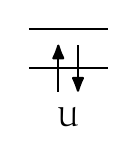
\begin{tikzpicture}
    \draw[thick] (0,0) -- (1,0);
    \draw[thick] (0,0.5) -- (1,0.5);
    
    \draw[-{Latex[round]}, thick] (0.375,-0.3) -- (0.375,0.3);
	\draw[{Latex[round]}-, thick] (0.625,-0.3) -- (0.625,0.3);
	
	\node at (0.5,-0.625) {$U$};
\end{tikzpicture}

% U'
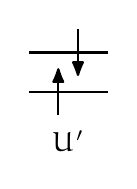
\begin{tikzpicture}
    \draw[thick] (0,0) -- (1,0);
    \draw[thick] (0,0.5) -- (1,0.5);
    
    \draw[-{Latex[round]}, thick] (0.375,-0.3) -- (0.375,0.3);
	\draw[{Latex[round]}-, thick] (0.625,0.2) -- (0.625,0.8);
	
	\node at (0.5,-0.625) {$U'$};
\end{tikzpicture}

% U'-J
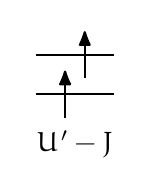
\begin{tikzpicture}
    \draw[thick] (0,0) -- (1,0);
    \draw[thick] (0,0.5) -- (1,0.5);
    
    \draw[-{Latex[round]}, thick] (0.375,-0.3) -- (0.375,0.3);
	\draw[-{Latex[round]}, thick] (0.625,0.2) -- (0.625,0.8);
	
	\node at (0.5,-0.625) {$U'-J$};
\end{tikzpicture}

% J
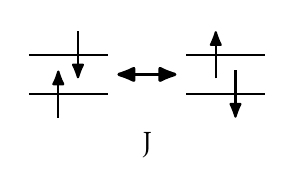
\begin{tikzpicture}
    \draw[thick] (0,0) -- (1,0);
    \draw[thick] (0,0.5) -- (1,0.5);
    
    \draw[-{Latex[round]}, thick] (0.375,-0.3) -- (0.375,0.3);
	\draw[{Latex[round]-}, thick] (0.625,0.2) -- (0.625,0.8);
	
	\draw[thick] (2,0) -- (3,0);
    \draw[thick] (2,0.5) -- (3,0.5);
    
    \draw[{Latex[round]-}, thick] (2.625,-0.3) -- (2.625,0.3);
	\draw[-{Latex[round]}, thick] (2.375,0.2) -- (2.375,0.8);
	
	\draw[-{Latex[round]}, very thick] (1.25,0.25) -- (1.875,0.25);
	\draw[-{Latex[round]}, very thick] (1.75,0.25) -- (1.125,0.25);
	
	\node at (1.5,-0.625) {$J$};
\end{tikzpicture}

% J
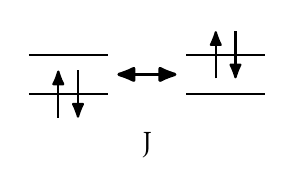
\begin{tikzpicture}
    \draw[thick] (0,0) -- (1,0);
    \draw[thick] (0,0.5) -- (1,0.5);
    
    \draw[-{Latex[round]}, thick] (0.375,-0.3) -- (0.375,0.3);
	\draw[{Latex[round]-}, thick] (0.625,-0.3) -- (0.625,0.3);
	
	\draw[thick] (2,0) -- (3,0);
    \draw[thick] (2,0.5) -- (3,0.5);
    
    \draw[{Latex[round]-}, thick] (2.625,0.2) -- (2.625,0.8);
	\draw[-{Latex[round]}, thick] (2.375,0.2) -- (2.375,0.8);
	
	\draw[-{Latex[round]}, very thick] (1.25,0.25) -- (1.875,0.25);
	\draw[-{Latex[round]}, very thick] (1.75,0.25) -- (1.125,0.25);
	
	\node at (1.5,-0.625) {$J$};
\end{tikzpicture}

\end{document}
